\cotefile{10}
\scanpage{115}
\mspage{114}


Chapter 1. Generalities on the operations $\unsure{\otimes|\Omega}$ on a category.

\inserted{\handwritten{Appendix: Review of coalgebras, comodules, bialgebras.....}}

Chapter 2. Relations between $\otimes$\deleted{-}categories \deleted{and} with fiber functor, and coalgebras resp. hyperalgebras: \deleted{Group} Tannaka duality.

\hfill (mi\rlap{c}xed structures, connections ....)

Chapter 3. \rlap{\raisebox{-1.2ex}{\tikz[x=1em,y=1em]{\draw (3,0)--(4.4,.8);}}}\uline{Numerous and varied examples.} \uline{Detailed dictionary.}

\margin{\handwritten{\figure{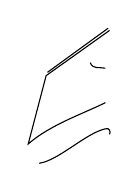
\begin{tikzpicture}[x=0.35cm,y=0.35cm]
\draw (2.9,4.8) -- (0.7,3.2);
\draw (2.95,4.72) -- (0.65,3.08) -- (0,0.6) .. controls (0.8,1.3) and (2,1.7) .. (2.8,2.1);
\draw (2.25,3.55) .. controls (2.35,3.3) and (2.55,3.4) .. (2.8,3.35);
\draw (0.4,-0.1) .. controls (1.1,0) and (2.1,1.0) .. (2.8,1.15) .. controls (2.95,1.2) and (3,1.05) .. (2.95,.95);
\end{tikzpicture}}}}
Chapter 4. Filtrations on a fiber functor.

Chapter 5. Structure theorem for $\otimes$-categories in terms of \rlap{G}gerbes.

Chapter 6. Polarization of a $\otimes$-category. Hodge groups.

Chapter 7. $\otimes$-Categories with reductive band. Classification over \uline{$R$}.

\unsure{\rlap{C}8|8|C}hapter 8. Ho\rlap{t}dge structures, Mumford-Tate groups and corresponding moduli spaces.

Chapter 9. Questions of effectivity (?)

\handwritten{Possibly a chapter by \unsure{Armature} on the ``\unsure{non-|non}commutative case''}

\handwritten{Another on \unsure{variants|variant|variant} for triangulated categories ?}

\handwritten{Chapter on Picard categories,(more generally\ groupoids with law $\otimes$) enveloping Picard categories. Case of categories having two law $\oplus$ and $\otimes$ ----}

\margin{\handwritten{\figure{\begin{tikzpicture}[x=1em,y=1em]
\draw (0,2.2) .. controls (.05,1.8) and (-.05,1.3) .. (.3,1.05) .. controls (.6,.9) and (.9,.85) .. (1,.95);
\draw (.85,0) .. controls (.95,-.2) and (1.03,-.3) .. (1.18,-.4);
\end{tikzpicture}}}}
